\documentclass[]{book}
\usepackage{textcomp}
\usepackage{gensymb}
\usepackage{graphicx}

%opening
\title{Orbital Mechanics for the\\ non-mathematically inclined}
\author{Derric Atzrott}

\begin{document}

\maketitle

\tableofcontents

\chapter{Introduction}

So for some reason you need to understand orbital mechanics, but you don't
consider yourself a math wiz.  I've been there.  This book, despite the
name, does include a great deal of math, but don't worry! I will teach
you everything you need to know in order to make sense of it.

This book will focus on what is called a two-body problem. This will
allow for a close approximation of the orbit of an object around a central
body. Technically since all objects with mass exert gravity on all other
objects with mass, the orbit of an object will be a little bit different,
but for most cases this will work, and the math is significantly easier.

I assume in this book that you have a basic high-school level understanding
of math.  You should be able to use a graphing calculator and understand
algebra.  In many cases I have already solved equations for the variables
that we are looking for, but if you want to know where these came from,
you should be able to do the algebra to figure that out.

I want this book to be useful for anyone who needs it, so it is being
made available under the Creative Commons Attribution Share-Alike license.
You can see the back of the book for the legalese of what that means, but
in a nutshell it means that you can make copies of this book to give to
your friends for free, and you are also allowed to make changes to this
book if you'd like!

If you have a little bit of money, I would greatly appreciate it if you'd
be willing to purchase this book, but if you don't then you shouldn't be
deprived of useful knowledge.  If you'd like to make modifications to the
book, please email me at \textit{zellfaze@zellfaze.org}.  I can send you
the \LaTeX\ source files for the book.  If you have any suggestions or
comments, you can also reach me at that email address.

\part{Required Background}

\chapter{Angles and Radians}

When most people think of angles they think of something that is measured in
degrees.

% Diagram showing small angle marked in degrees
\bigskip
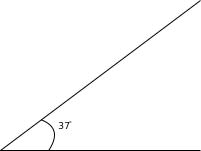
\includegraphics[width=1.5in]{images/angledegree}
\bigskip


Most people also would know that there are 360\textdegree\ in a circle

% Diagram showing a circle with varius angles marked in degrees
\bigskip
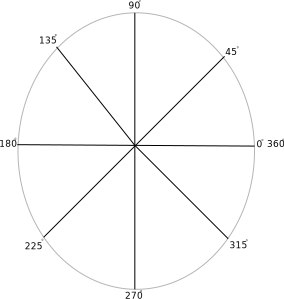
\includegraphics[width=2.5in]{images/circledegree}
\bigskip

While this is a useful way to look at angles for people, for various reasons
it is not a very good way to measure angles when working in a mathematical
setting.  Instead a unit known as Radians is used to measure angles.
There are a total of $2\pi$ radians in a circle.

% Diagram showing circle with varius angles marked in radians
\bigskip
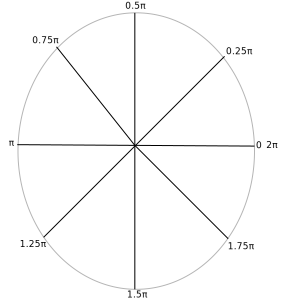
\includegraphics[width=2.5in]{images/circleradian}
\bigskip

Thankfully, it is easy to convert between radians and degrees. The formula
for that is:

% Formula for degrees to radians
\bigskip
$degrees = \frac{radians}{\pi/180}$

% Formula for radians to degrees
\bigskip
$radians = degrees*\pi/180$
\bigskip

For the rest of this document we will be using radians, not degrees, to
measure angles. You can always refer back to the above formulas for
converting between the two if needed.

\chapter{Basic Trigonometry}

A lot of orbital mechanics requires the use of some basic trigonometry to
calculate.  In this chapter we are going to cover the concepts required.

There are six different trigonometric functions that are you will need to
know.  These are sine, cosine, and tangent, along with arcsine, arccosine,
and arctangent.  These are usually abbreviated as sin, cos, tan, arcsin,
arccos, and arctan respectively. You will also need to know the Pythagorean Theorem.

To explain these lets start by drawing a right triangle (a triangle where
one of the angles is $0.5\pi$ radians).

% Diagram showing labeled right triangle
\bigskip
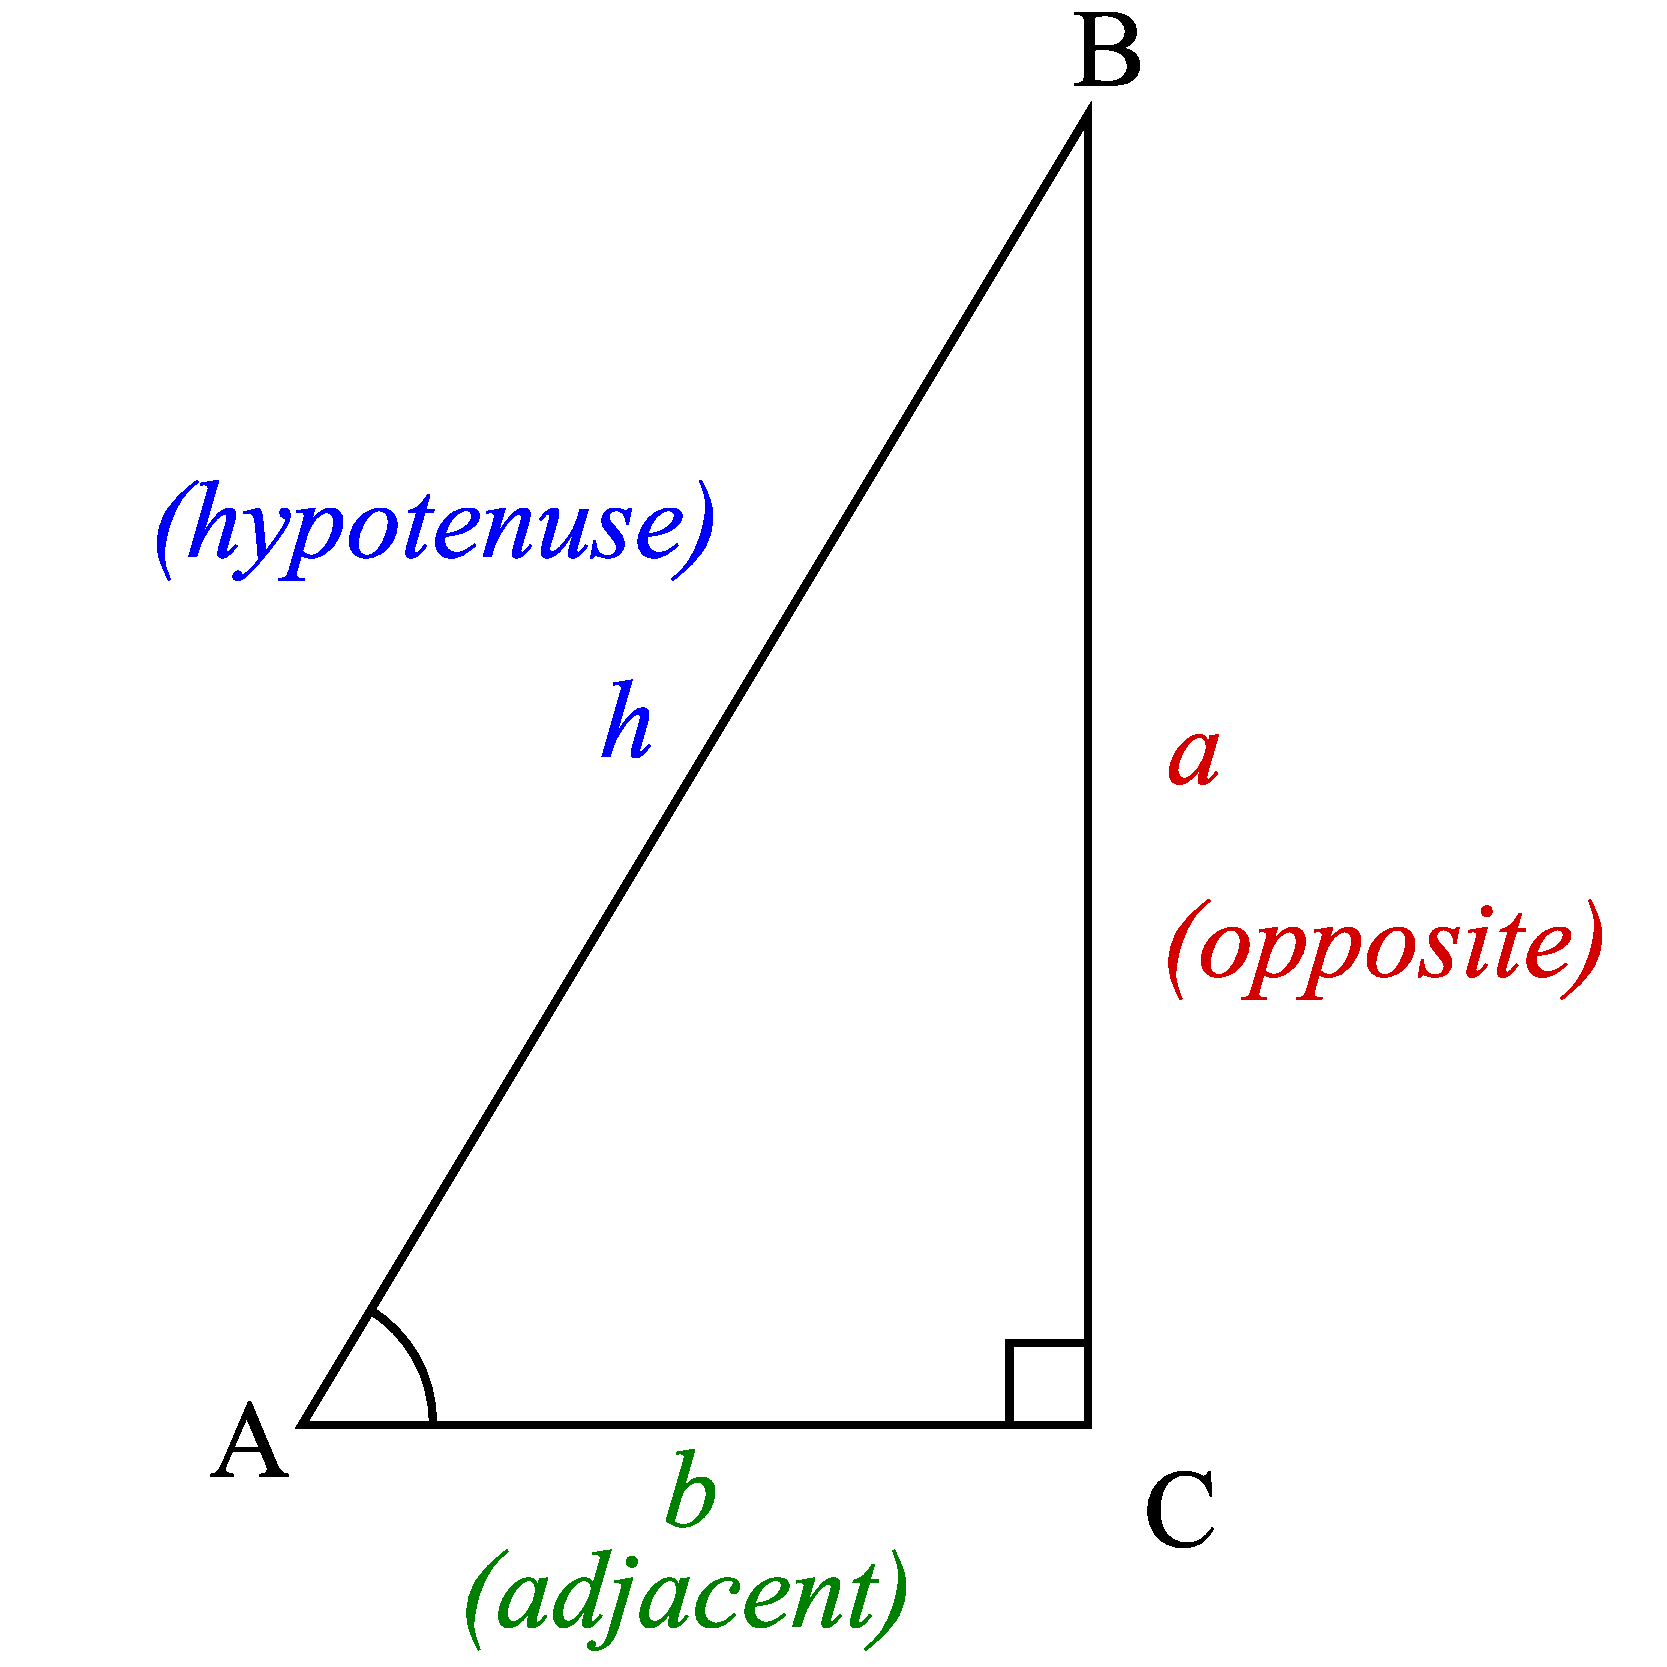
\includegraphics[width=3in]{images/Trigonometry_triangle}

\textit{Credit: Tarquin of en.wp CC-BY-SA 3.0 Unported}
\bigskip

\section{Calculating Angles}

All of the angles in a triangle will always add up to $\pi$ radians.
Knowing this, if you know two of the angles of a triangle, you can always
find the third.

% Formula for radians to degrees
\bigskip
$\pi = A+B+C$
\bigskip

\section{Calculating Sides}

The Pythagorean Theorem provides a similar formula for finding the length 
of any of the sides if you know the length of other two.

\bigskip
$h^2 = a^2 + b^2$
\bigskip

We can rearrange this equation for if we need to find a or b given h and
the remaining side.

\bigskip
$a = \sqrt{h^2 -b^2}$

\bigskip
$b = \sqrt{h^2 -a^2}$
\bigskip

\section{Trigonometric Functions}

Alright, so we now know how to find the last angle in a triangle if we
have the other angles, and how to find the last side length if we have
the other side lengths.  We also though need to be able to find angles
given the length of a side and how long the sides are given some of the 
angles in a triangle.  These are both found using the six trigonometric
functions.

The first three of the trigonometric functions allow you to find the ratio
between two of the sides of the triangle if you know one of the angles. In
this case, we will assume that we know angle A, but you could change this
to knowing angle B with a little reworking.

\bigskip
$\sin{A} = \frac{a}{h}$
\bigskip

$\cos{A} = \frac{b}{h}$
\bigskip

$\tan{A} = \frac{a}{b}$
\bigskip

Your calculator should be able to find the sin, cos, or tan for any given
number.  It is worth knowing that sin or cos values will always be
between -1 and 1.  A tan value will never be equal to $\pm \frac{x\pi}{2}$,
where x is an odd number. Thus $\pm\frac{\pi}{2}$ and $\pm\frac{3\pi}{2}$
are invalid for tangents. Otherwise all numbers are valid for tangents.
The reason for this is not really needed to continue so we won't be getting
into it.

Somewhat more obviously useful is to take the side lengths and go the other
direction.  It is easy to find the ratio between two sides of a triangle
and we can use that information to find an angle.  To do this we use arcsin,
arccos, and arctan which cancel out sin, cos, and tan respectively.

\bigskip
$A = \arcsin{\frac{a}{h}}$
\bigskip

$A = \arccos{\frac{b}{h}}$
\bigskip

$A = \arctan{\frac{a}{b}}$
\bigskip

You now know enough trigonometry in order to understand orbital mechanics.

\chapter{Vectors}

A vector is simply a line segment with a magnitude (aka a length) and a
direction (which is just an angle).  You can define a vector with its
magnitude and direction, but in many cases it is easier to define a vector
in terms of coordinates instead.  These coordinates are often called the x
and y components of the vector.

For example, a vector that is defined as \{10,15\} is a line segment from
\{0,0\} to the coordinate \{10,15\}.  Since vectors are technically just a
magnitude and a direction, all vectors defined by coordinates originate
at \{0,0\}.

% Diagram showing simple vector
\bigskip
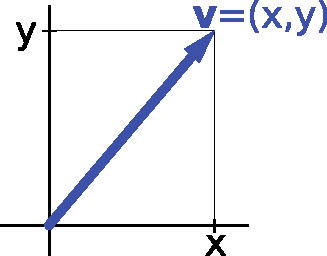
\includegraphics[width=2in]{images/Vector_components}

\textit{Credit: Jakob.scholbach of Wikimedia Commons CC-BY-SA 3.0 Unported}
\bigskip

The direction of the vector is the angle made by the vector line and the
x axis.  The magnitude is the length of the vector line.

\section{Comparing Vectors}

Two vectors are considered to be equal if their direction and magnitude are
the same.  Vectors that are opposite of each other have the same magnitude,
but are pointed in the exact opposite directions.  Parallel vectors have
the same direction, but different magnitudes.

\section{Finding Magnitude and Direction}

You can find the magnitude of a vector from its coordinates with this
formula:

\bigskip
$magnitude = \sqrt{x^2+y^2} $
\bigskip

You can find the direction of a vector from its coordinates with this
formula:

\bigskip
$direction = \arctan{\frac{y}{x}} $
\bigskip

\section{Vector Arithmetic}

You can perform a number of operations on vectors. We will be covering the
most common types.

\subsection{Basic Operations}

Vectors can be added together by adding their coordinates together.  For
example:

\bigskip
$\{5,5\} = \{1,3\} + \{4,2\}$
\bigskip

Subtraction works in the exact same way.

\bigskip
$\{4,2\} = \{5,5\} - \{1,3\}$
\bigskip

You can multiple a vector by a number (also sometimes called a scalar) by
multiplying each of the vectors components with the number.

\bigskip
$\{4,8\} = \{2,4\} * 2$
\bigskip

Division works in the exact same way.

\bigskip
$\{2,4\} = \{4,8\} / 2$
\bigskip

\subsection{Dot Product}
A dot product is sort of like multiplication for two vectors, except that
it leaves you with a single number when you are done instead of a new
vector. It is relatively easily done.

Let's say that you have two vectors we'll call them $V_{1}$ and $V_{2}$.
We will define them as follows.

\bigskip
$V_{1} = \{2,4\}$

$V_{2} = \{3,5\}$

\bigskip
You can calculate their dot product by multiplying their components
together and then adding the resulting components. See the following
example:

\bigskip
$V_{1} \bullet V_{2} = (2*3)+(4*5) = 26$

\bigskip

More generally you could define it as:

\bigskip
$V_{1} \bullet V_{2} = (X_{1}*X_{2})+(Y_{1}*Y_{2})$

\subsection{Cross Product}

Like dot products, cross products could also be considered something like
multiplication.  Unlike dot products, the cross product of two vectors
is a third vector.  Cross products can't be done on 2D vectors, so for the
first time, we will be using a 3D vector.  Things work just the same for
3D vectors, just we have an additional coordinate. (They also have an
additional direction angle, but we won't need that here.)

You can calculate their cross product using the following formula:

\bigskip
$V_{1}$ \texttimes\ $V_{2} = $

$X_{3} = Y_{1}*Z_{2} - Z_{1}*Y_{2}$

$Y_{3} = Z_{1}*X_{2} - X_{1}*Z_{2}$

$X_{3} = X_{1}*Y_{2} - Y_{1}*X_{2}$
\bigskip

How about an example? Let's define two vectors again. Again we'll call them 
$V_{1}$ and $V_{2}$.

\bigskip
$V_{1} = \{2,4,6\}$

$V_{2} = \{3,5,7\}$

\bigskip

$V_{1}$ \texttimes\ $V_{2} = $

$X_{3} = 4*7 - 6*5 = -2$

$Y_{3} = 6*3 - 2*7 = 4$

$X_{3} = 2*5 - 4*3 = -2$

\bigskip

$V_{1}$ \texttimes\ $V_{2} = \{-2,4,-2\}$
\bigskip

One of the cool things about cross products is their relationship to each
other.  They are sort of like the angles or sides of a triangle in that if
you know two of them, you can always find the third.  They have the
following relationship:

\bigskip
$V_{3} = V_{1}$ \texttimes\ $V_{2}$

$V_{2} = V_{1}$ \texttimes\ $V_{3}$

$V_{1} = V_{2}$ \texttimes\ $V_{3}$
\bigskip

\part{Orbital Mechanics}

\chapter{Keplerian Orbital Elements}

There are many ways to define the orbit of an object, but the one that
allows one to most easily see the shape of the orbit itself are the
Keplerian Orbital Elements.  The other methods of defining an orbit's
shape can all be calculated from these, so it is with these that we will
start.

Below I have included a diagram showing some of the orbital elements. This
is provided so that you may get a general summary of what is to follow.

% Diagram showing overview of keplerian elements
\bigskip
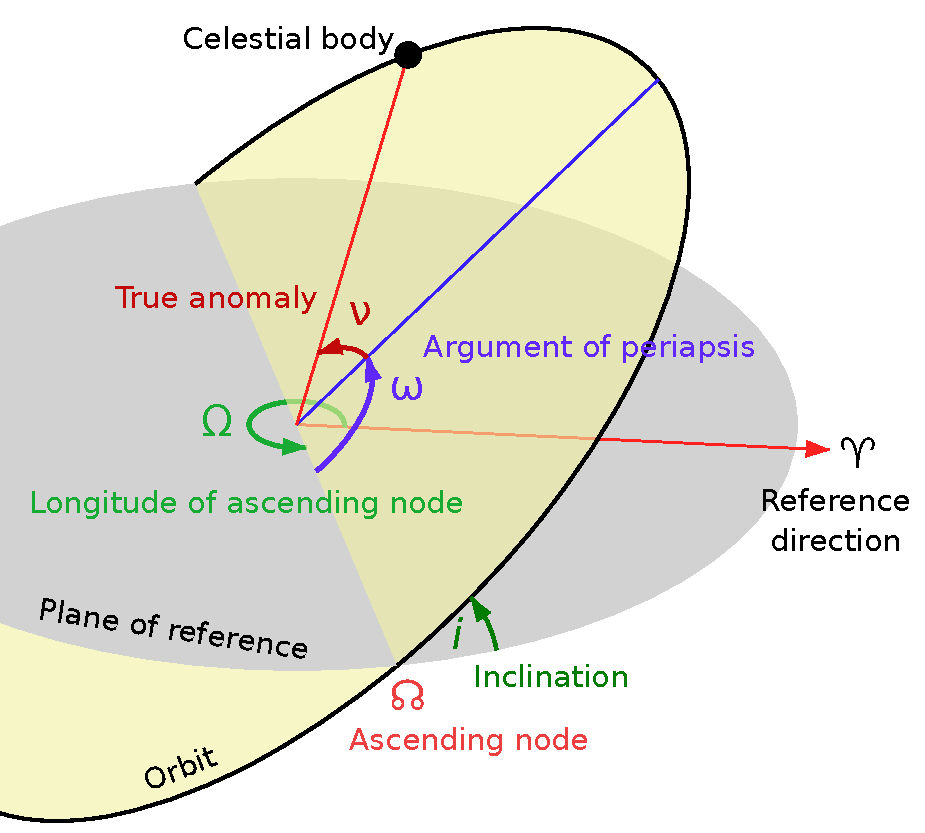
\includegraphics[width=3.5in]{images/Orbit1}

\textit{Credit: Lasunncty of Wikimedia Commons CC-BY-SA 3.0 Unported}
\bigskip

\section{Eccentricity}

Eccentricity is the orbital element that describes the shape of the curve
that the orbit takes.  It describes the shape of the orbit, but not the
orbit's position, the position of the central body, or the position of
the orbiting object.

The eccentricity of an orbit can never be negative.  An eccentricity of
0 describes an orbit that is perfectly circular.  The higher the
eccentricity the less like a circle and the more like a line the orbit is.

An eccentricity value greater than 0 but less than 1 is an ellipse. If
eccentricity is 1 then it is a parabola, and if eccentricity is greater
than 1 then it is a hyperbola.  Parabolic and hyperbolic orbits do not
form a closed loop.

% Diagram showing overview of keplerian elements
\bigskip
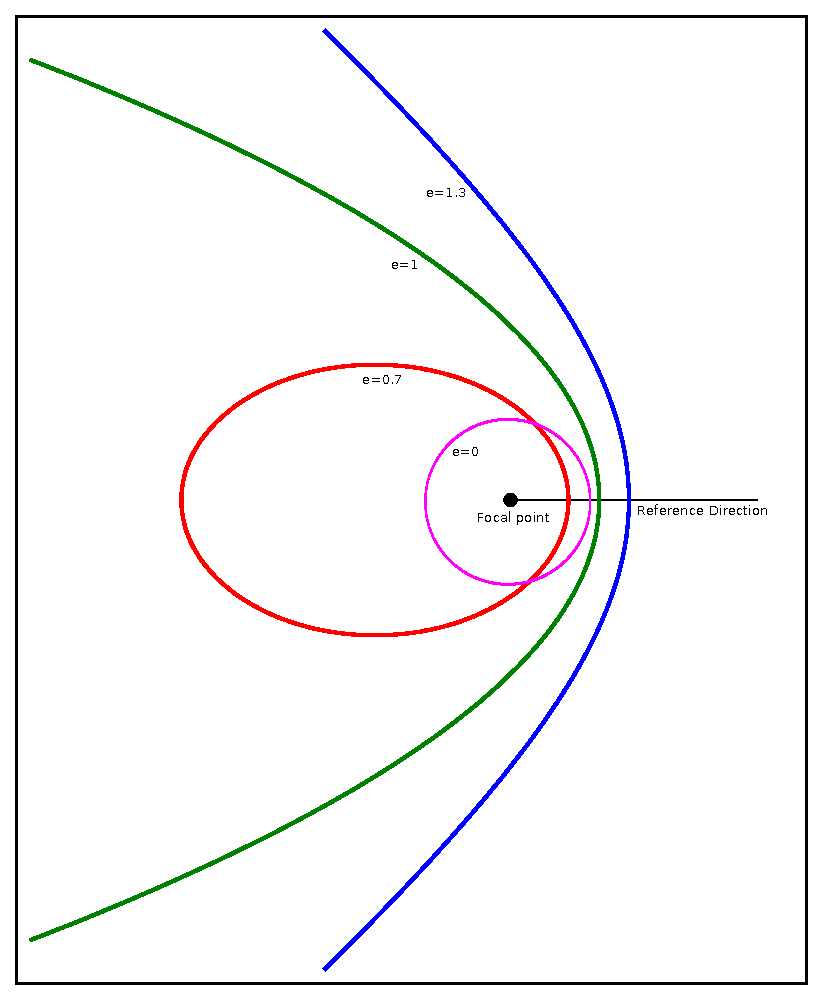
\includegraphics[width=4in]{images/Kepler_orbits}

\textit{Credit: Based off work by Stamcose of Wikimedia Commons CC-BY-SA 3.0 Unported}
\bigskip

\section{Semi-Major Axis}

Along with the eccentricity, the semi-major axis also describes the shape
of an orbit.  In a circular orbit the semi-major axis is the radius of the
circle.  In an elliptical orbit, it is half the distance between the two
farthest points.  In a parabolic or hyperbolic orbit, it is the distance
between the central body and the closest approach of the orbiting body.

% Diagram showing semi-major axis labeled on circle

% Diagram showing semi-major axis labeled on ellipse

% Diagram showing semi-major axis labeled on parabola

\section{Inclination}

\section{Longitude of the Ascending Node}

\section{Argument of Periapsis}

\section{The Anomalies}

\subsection{Mean Anomaly}

\subsection{True Anomaly}

\subsection{Eccentric Anomaly}

\end{document}
